%%%%%%%%%%%%%%%%%%%%%%%%%%%%%%%%%%%%%%%%%%%%%%%%%%%%%%%
%                   File: OSAmeetings.tex             %
%                  Date: March 21, 2007  MSD          %
%                                                     %
%     For preparing LaTeX manuscripts for submission  %
%       submission to OSA meetings and conferences    %
%                                                     %
%       (c) 2007 Optical Society of America           %
%%%%%%%%%%%%%%%%%%%%%%%%%%%%%%%%%%%%%%%%%%%%%%%%%%%%%%%

\documentclass[letterpaper,10pt]{article}
\usepackage{osameet2}

%% standard packages and arguments should be modified as needed

\usepackage{amsmath,amssymb}

% \bibliography{paper}
% \bibliographystyle{osajnl}


%\usepackage[pdftex,colorlinks=true,bookmarks=false,citecolor=blue,urlcolor=blue]{hyperref} %pdflatex
\usepackage[colorlinks=true,bookmarks=false,citecolor=blue,urlcolor=blue]{hyperref} %latex w/dvips


\begin{document}

\title{Three-dimensional fluorophore orientation imaging with polarized multiview microscopy}

\author{Talon Chandler,${}^{1,*}$ Min Guo,${}^2$ Shalin Mehta,${}^{1,3,4}$ Abhishek Kumar,${}^2$\\ Hari Shroff,${}^{2,5}$ Rudolf Oldenbourg,${}^{3,6}$ Patrick J. La Rivi\`ere${}^{1,5}$}

\address{${}^1$Department of Radiology, University of Chicago, Chicago, Illinois 60637, USA.\\ ${}^2$Section on High Resolution Optical Imaging, National Institute of Biomedical Imaging\\ and Bioengineering, National Institutes of Health, Bethesda, Maryland 20892, USA.\\ ${}^3$Bell Center, Marine Biological Laboratory, Woods Hole, Massachusetts 02543, USA.\\ ${}^4$(present address) Chan Zuckerberg Biohub, San Francisco, California 94158, USA.\\ ${}^5$Whitman Center, Marine Biological Laboratory, Woods Hole, Massachusetts 02543, USA.\\ ${}^6$Department of Physics, Brown University, Providence, Rhode Island 02912, USA.}
\email{${}^*$talonchandler@talonchandler.com} %% email address is required

\begin{abstract}
  \hspace{-0.75em} We show that polarized fluorescence microscopes make band-limited measurements
  in the angular frequency domain. We use this result to propose and demonstrate
  efficient algorithms for reconstructing three-dimensional fluorophore
  orientations from polarized multiview microscope data.
\end{abstract}

\ocis{180.2520 Fluorescence microscopy, 260.5430 Polarization}

\section{Introduction}
Polarized fluorescence microscopes can measure the orientation of fluorophores
in live specimens\cite{weiss1999}. Unfortunately, existing techniques are
limited to imaging two-dimensional orientations in thin samples, and attempts to
generalize these approaches to three-dimensional orientations have faced
computational difficulties. We propose the use of the spherical harmonics to
simplify the analysis of polarized fluorescence microscopes. In the same way
that the Fourier transform simplifies the analysis of spatial imaging systems,
the spherical Fourier transform simplifies the analysis of angular imaging
systems.

\section{Theory}
Consider a small volume that contains many non-interacting fluorophores. We
define the orientation distribution function $f(\hat{\mathbf{r}})$ as the number
of fluorophores per steradian oriented in a direction $\hat{\mathbf{r}}$. The
goal of polarized fluorescence microscopy is to estimate $f(\hat{\mathbf{r}})$
in many volumes throughout a three-dimensional sample.

The forward model for an $N$-measurement polarized fluorescence microscope is
given by
\begin{align}
  g_i = \int_{\mathbb{S}^2}d\hat{\textbf{r}}\ h_i(\hat{\textbf{r}})f(\hat{\textbf{r}})\hspace{1em}\text{for}\hspace{1em} i=1,\dotsc,N
\end{align}
where $h_i(\hat{\textbf{r}})$ is the point response function of the $i$th
microscope configuration, the integral is over the sphere $\mathbb{S}^2$, and
$g_i$ is the $i$th intensity measurement. By discretizing $f(\hat{\mathbf{r}})$
and expanding $h(\hat{\mathbf{r}})$ in terms of the spherical harmonics, we can
rewrite Equation~1 as
\begin{align}
  \mathbf{g} = \Psi\hspace{0.1em}\mathbf{B}^+\mathbf{f}
\end{align}
where $\mathbf{f} = [f(\hat{\mathbf{r}}_1), \cdots, f(\hat{\mathbf{r}}_R)]^T$ is
a vector of $R$ samples of $f(\hat{\mathbf{r}})$; $\mathbf{B}$ is a matrix of
the spherical harmonics evaluated at the sample points,
$\mathbf{B}_{ij} = Y_j(\hat{\mathbf{r}}_i)$ where $Y_j$ is the $j$th spherical
harmonic; $\cdot^+$ is the Moore-Penrose pseudoinverse; $\Psi$ is a matrix of
the spherical harmonic coefficients of the point response functions,
$\Psi_{ij} = \int_{\mathbb{S}^2}d\hat{\textbf{r}}\
h_i(\hat{\mathbf{r}})Y_j(\hat{\mathbf{r}})$; and
$\mathbf{g} = [g_1, \cdots, g_N]^T$ is a vector of the $N$ intensity
measurements.

The point response functions for a wide class of polarized fluorescence
microscopes have been calculated previously\cite{chandler}. For many polarized
fluorescence microscopes the point response function can be expanded in terms of
a small number of spherical harmonics. If the point response functions can be
expanded in terms of $M$ spherical harmonics then $\Psi$ is an $N\times M$
matrix and $\mathbf{B}^+$ only needs to be calculated in the first $M$
columns. This simplification reduces Equation 1 from a set of integrals to an
efficient series of matrix multiplications.

\section{Methods and Results}
We labeled the actin filaments of a fixed-cell sample with Alexa Fluor 488
Phalloidin and imaged the sample with an asymmetric 1.1/0.71 NA dual-view
inverted selective plane illumination microscope\cite{wu2017} with variable
polarizers added to both illumination paths. The dipole moment of Alexa Fluor
488 Phalloidin is known to align parallel to the long axis of actin filaments,
so this sample makes a suitable test specimen for our reconstruction
algorithm. We imaged the specimen volume eight times---two views with four
illumination polarization orientations each.

To reconstruct the orientation in each voxel we solved the following problem 
\begin{align}
\mathbf{f^{\thinspace *}}= \underset{\mathbf{f}\in\{\mathbf{e}_i\}\ i = 0,\dotsc,R}{\text{argmin}}
\ \ ||\thinspace\mathbf{g} - \Psi\hspace{0.1em}\mathbf{B}^+\mathbf{f}\thinspace||_2^2
\end{align}
where $\mathbf{e}_i$ is a vector with a one in the $i$th entry and zeros
elsewhere. By constraining $\mathbf{f}$ we are assuming that all of the
fluorophores in each voxel are oriented in the same direction---a reasonable
assumption for this sample.

\begin{figure}[htbp]
  \centering
  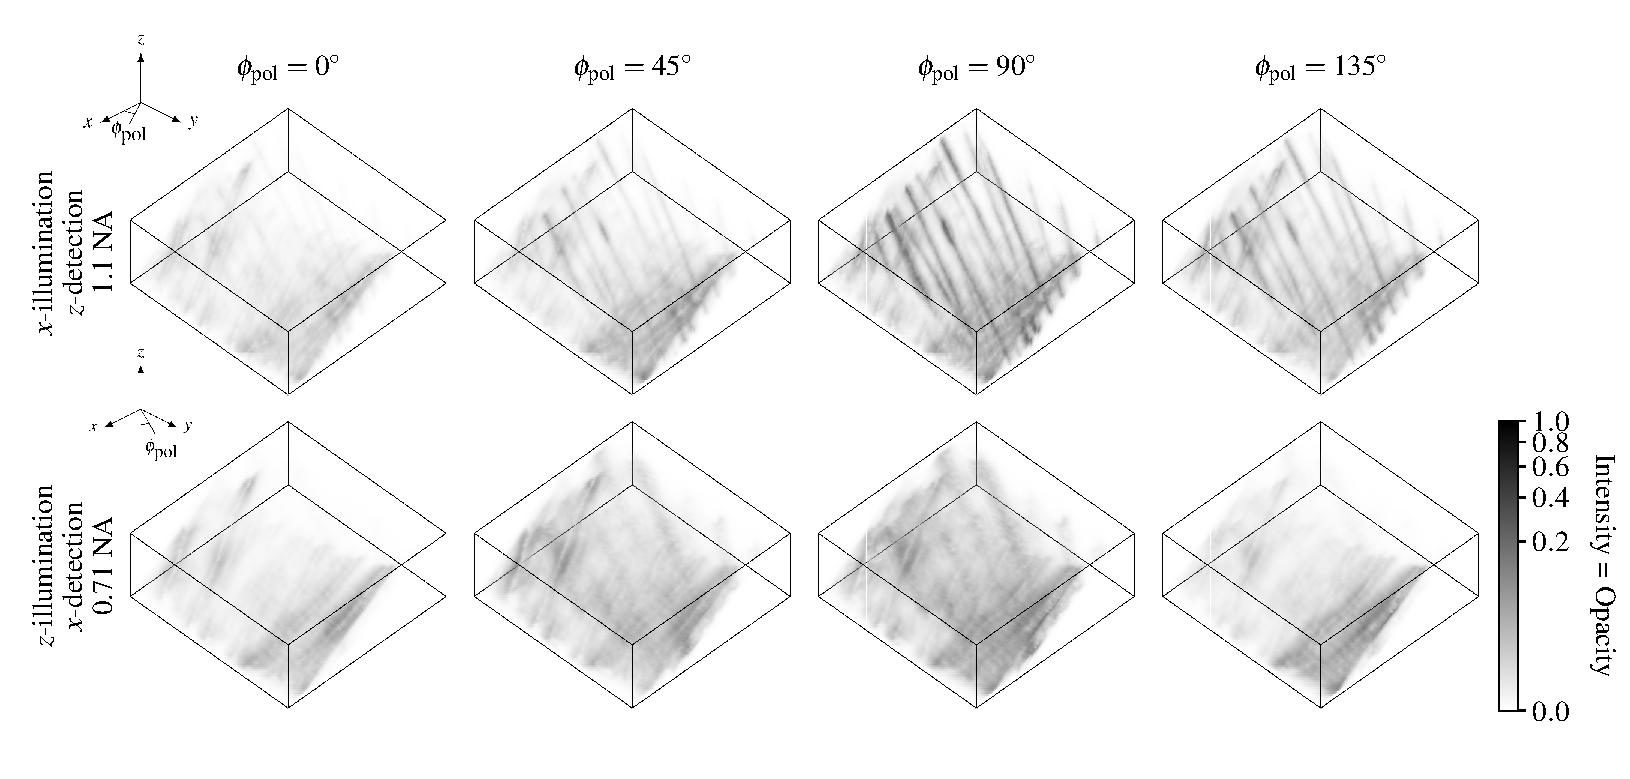
\includegraphics[width=16.cm, trim={0.1cm 1.3cm 0 0.5cm}]{figs/roi2/data.pdf}
  \caption{Intensity data from a $13.5\times 13.5\times 5.4\ \mu$m${}^3$ volume
    from two views (rows) and four illumination polarization orientations
    (columns).}
\end{figure}
\vspace{0.1em}
\begin{figure}[htbp]
  \centering
  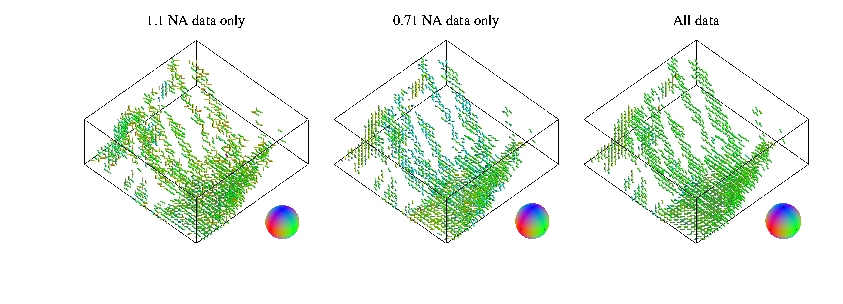
\includegraphics[width=16.0cm, trim={1cm 1.2cm 0 0.8cm}]{figs/roi2/recon.pdf}
  \caption{Orientation reconstructions using (left) only data from the 1.1 NA
    view, (center) only data from the 0.71 NA view, and (right) data from both
    views. Data from both views is required to correctly reconstruct the
    three-dimensional orientation of fluorophores.}
\end{figure}
\vspace{-2.5em}
{\footnotesize\bibliography{abstract}{}}
\bibliographystyle{osajnl}

\end{document}
